\documentclass[12pt,a4paper]{article}

\usepackage[utf8x]{inputenc}
\usepackage[english]{babel}
\usepackage{xcolor}
\usepackage{hyperref}
\usepackage{parskip}
\usepackage{graphicx}
\usepackage{listings} % For code snippets
\usepackage{xcolor}
\usepackage[left=2cm, top=3cm, text={17cm, 24cm}]{geometry} 

\newcommand{\todo}[1]{\noindent\textcolor{red}{[[\textbf{TODO} \textbf{#1]]}}\\}
\newcommand{\phony}[1]{\textcolor{gray}{#1} \\}

\definecolor{codegreen}{rgb}{0,0.6,0}
\definecolor{codegray}{rgb}{0.5,0.5,0.5}
\definecolor{codepurple}{rgb}{0.58,0,0.82}
\definecolor{backcolour}{rgb}{0.95,0.95,0.92}

% Setup for code snippets
\lstdefinestyle{mystyle}{
    backgroundcolor=\color{backcolour},   
    commentstyle=\color{codegreen},
    keywordstyle=\color{magenta},
    numberstyle=\tiny\color{codegray},
    stringstyle=\color{codepurple},
    basicstyle=\ttfamily\footnotesize,
    breakatwhitespace=false,         
    breaklines=true,                 
    captionpos=b,                    
    keepspaces=true,                 
    numbers=left,                    
    numbersep=5pt,                  
    showspaces=false,                
    showstringspaces=false,
    showtabs=false,                  
    tabsize=4
}

% Path to images
\graphicspath{ {./images/} } 

% Setup for hyperrefs
\hypersetup{
    colorlinks=true,
    linkcolor=blue,
    filecolor=magenta,      
    urlcolor=blue,
}

% Globally disable indentation -> package parskip
\setlength{\parindent}{0pt}

\begin{document}
    \begin{titlepage}
        \begin{center}
            \vspace*{1cm}
    
            \Large{\textbf{Simulation of T-type crossroad \\ on FRDM-KL27z board}}
    
            \vspace{0.5cm}
            Project IMP\\
            Brno University of Technologies
            \vspace{1.5cm}
            
            
            \vfill
                
            \vspace{0.8cm}
        
            \textbf{Pavel Yadlouski (xyadlo00)}\\
            September, 2020
            
        \end{center}
    \end{titlepage}
    
    \tableofcontents
    \newpage

    \section{Introduction}
    Aim of this project is to implement an algorithm for controlling traffic lights at an intersection with pedestrian crossings of "request" type.
    Traffic lights are represented by LEDs on shield with schematic representation of T-type intersection.
    For each pedestrian crossing there is button.
    Signal from button represents that pedestrian came to crossing and send request for crossing the road by pressing on corresponding button.
    Shield with LEDs and buttons is connected to FRDM-KL27z board.
    
    \section{Architecture}
    Intersection is divided into 3 logical parts: bottom, central and top part.
    \begin{figure}[h!]
        \centering
        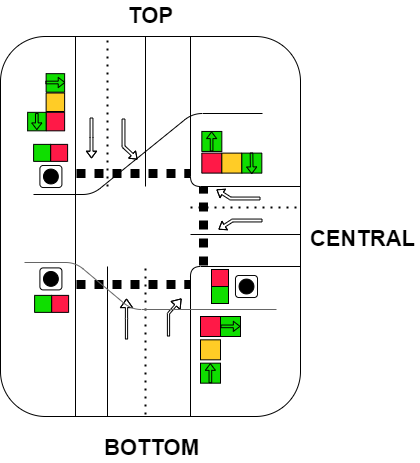
\includegraphics[scale=0.5]{images/semaphore.png}
        \caption{Logical division of intersection}
        \label{fig:my_label}
    \end{figure}
    
    \noindent In initial state bottom and top traffic lights are red and central traffic light has both green LEDs on.
    Check for any request is handled before starting new cycle.
    Cycle include sequence of steps from the initial state to the opposite side of semaphore and back to the initial state.
    Also any handler of interrupts ends in this initial state.
    The reason for this is that function for processing corresponding combination of buttons are called before new cycle, so loop can continue from initial state after request processing.
    One cycle in total takes 18 seconds.
    Taking one traffic light as an example:
    \begin{enumerate}
        \item 6 seconds in red
        \item 3 seconds in orange
        \item 6 seconds in green
        \item 3 seconds in orange
    \end{enumerate}

    \section{Implementation}
    In main infinite loop of the program there is switching of all car traffic lights.
    For switching light on individual traffic light there are 4 functions.
    Each function switch light from one light to the next in corresponding order.
    \begin{enumerate}
        \item red $\rightarrow$ orange -- \textit{change\_red\_orange\_\textbf{side}()}
        \item orange $\rightarrow$ green -- \textit{change\_orange\_green\_\textbf{side}()}
        \item green $\rightarrow$ orange -- \textit{change\_green\_orange\_\textbf{side}()}
        \item orange $\rightarrow$ red -- \textit{change\_orange\_red\_\textbf{side}()}
    \end{enumerate}
    where \textit{\textbf{side}} is one of three available sides: bottom, central or top.
    Each function contains simple setting and clearing bits of LEDs in corresponding registers.
    In functions \textit{change\_orange\_green\_\textbf{side}()} there is switch case that enables both green LEDs or only one of them based on its argument \textit{arrow}.
    
    \subsection*{Interrupts handling}
    When interrupts came, program switch to handler \textit{PORTB\_PORTC\_PORTD\_PORTE\_IRQHandler()}.
    In this handler flag for corresponding button is set.
    Flags is a boolean value \textit{\textbf{side}\_button}
    So, during any cycle this flags can be set.
    When system is in initial state before next standard cycle based on combination of button flags appropriate function is called.
    Every function for processing this kind of request has name in format \textit{handler\_\textbf{side}()}.
    Here \textit{\textbf{side}} means any combination of three sides (bottom, central, top) where button is placed (e.g \textit{handler\_bottom\_top()} means handler for request from bottom and top buttons simultaneously)
    
    \section{Problems and limitations}



\end{document}